\section{Validaci\'on}

La verificaci\'on del modelo propuesto comienza con la simulaci\'on num\'erica de los problemas utilizados hasta esta etapa. Por un lado, se llev\'o a cabo la resoluci\'on del problema de construcci\'on de Maxwell en una cavidad c\'ubica, destinada a verificar el tratamiento de la inconsistencia termodin\'amica por parte del modelo de Xu. Por otro lado, se verific\'o la capacidad de la \lbe{} propuesta para reproducir adecuadamente la transferencia de calor en un fluido van der Waals estratificado y en el avance de un frente de evaporaci\'on.

\red{Poner que el modelo de Xu isot\'ermico ya est\'a validado en varios trabajos, as\'i que ac\'a s\'olo se verifica la implementaci\'on y se resuelven los problemas anal\'iticos}


\subsection{Construcci\'on de Maxwell} 

La base de un problema de construcci\'on de Maxwell es similar a la utilizada en el \chap{chap:isot}, y consiste en simular la evoluci\'on de un fluido en condiciones de saturaci\'on dentro de una cavidad peri\'odica, comparando las densidades reproducidas dentro de cada fase con aquellas determinadas por la ecuaci\'on de estado utilizada. En este caso, el dominio simulado consiste en una cavidad c\'ubica de $100 \times 100 \times 100$ unidades de grilla, con condiciones de contorno peri\'odicas, temperatura uniforme, sin fuerzas externas, y que inicialmente contiene un fluido ven der Waals con densidad perturbada aleatoriamente en  $\pm 1\%$ alrededor del valor cr\'itico ($\rho=\rho_c$). Como se ejemplifica en la \fig{fig:maxwell_3d}, en los primeros instantes comienzan a generarse regiones de diferente densidad, que contin\'uan separ\'andose y agrup\'andose hasta formar estructuras con densidades claramente diferentes. De esta manera, pueden tomarse los valores de densidad en el interior de cada fase, lejos de las interfases, y compararlos con los determinados por la regla de Maxwell.

\begin{figure}[htb]
    \centering
    \begin{subfigure}[t]{0.45\textwidth}
        \centering
        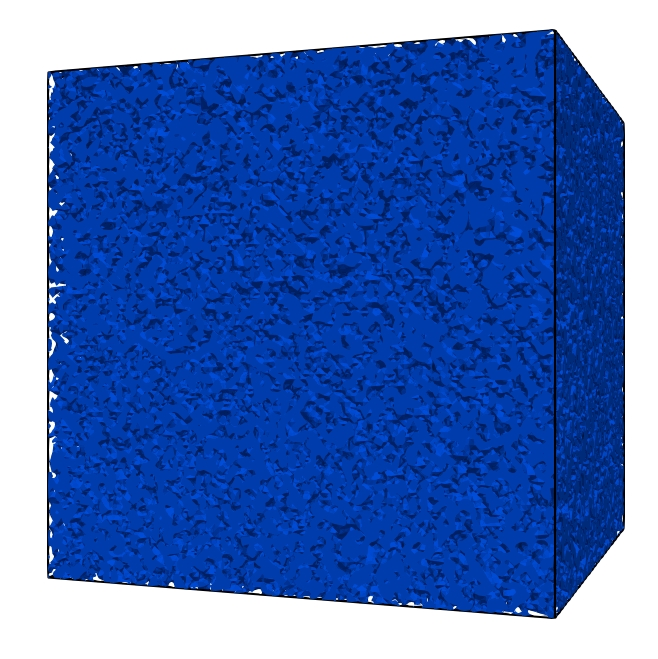
\includegraphics[width=0.95\textwidth]{Imagenes/Maxwell3D/Maxwell3D_sim/Imagenes/t_0}
        \caption{$t=0$}
    \end{subfigure}
    \begin{subfigure}[t]{0.45\textwidth}
        \centering
        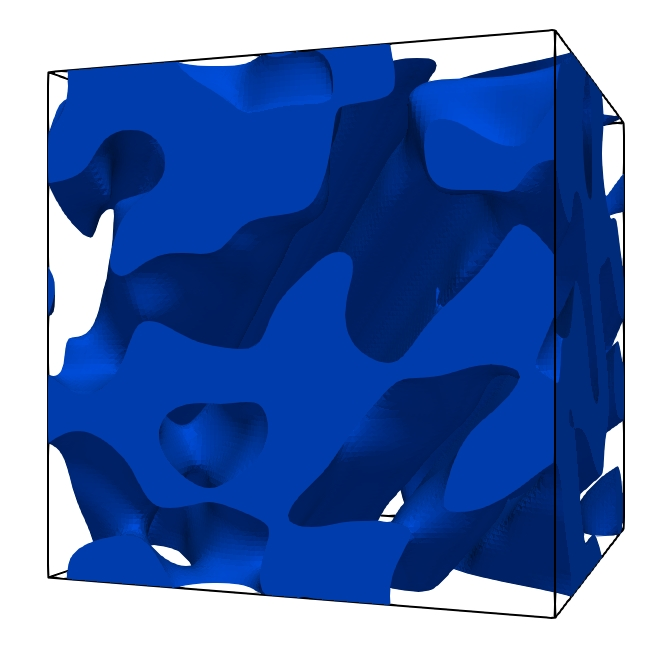
\includegraphics[width=0.95\textwidth]{Imagenes/Maxwell3D/Maxwell3D_sim/Imagenes/t_100}
        \caption{$t = 100$}
    \end{subfigure}
    \begin{subfigure}[t]{0.45\textwidth}
        \centering
        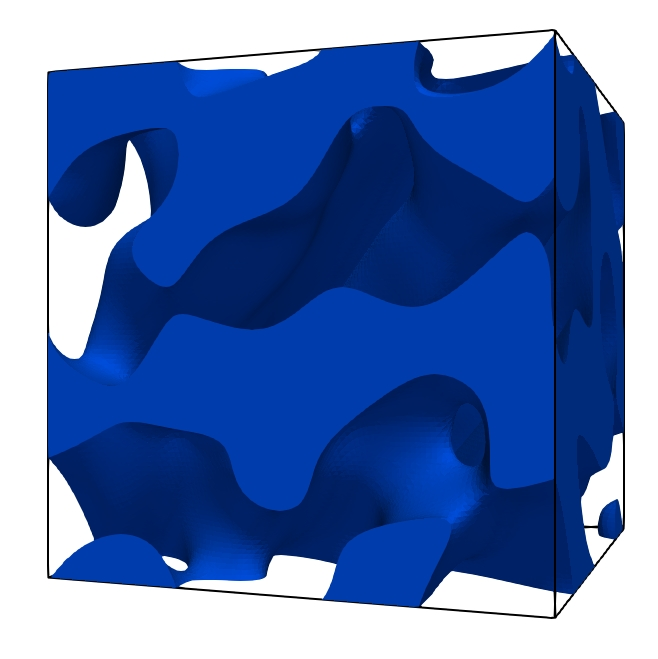
\includegraphics[width=0.95\textwidth]{Imagenes/Maxwell3D/Maxwell3D_sim/Imagenes/t_500}
        \caption{$t = 500$}
    \end{subfigure}    
    \begin{subfigure}[t]{0.45\textwidth}
        \centering
        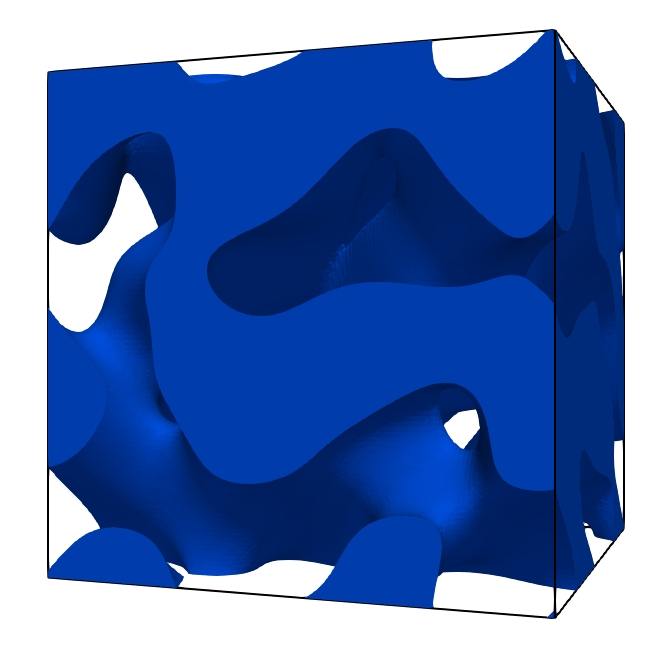
\includegraphics[width=0.95\textwidth]{Imagenes/Maxwell3D/Maxwell3D_sim/Imagenes/t_1000}
        \caption{$t = 1000$}
    \end{subfigure}    
    \begin{subfigure}[t]{0.45\textwidth}
        \centering
        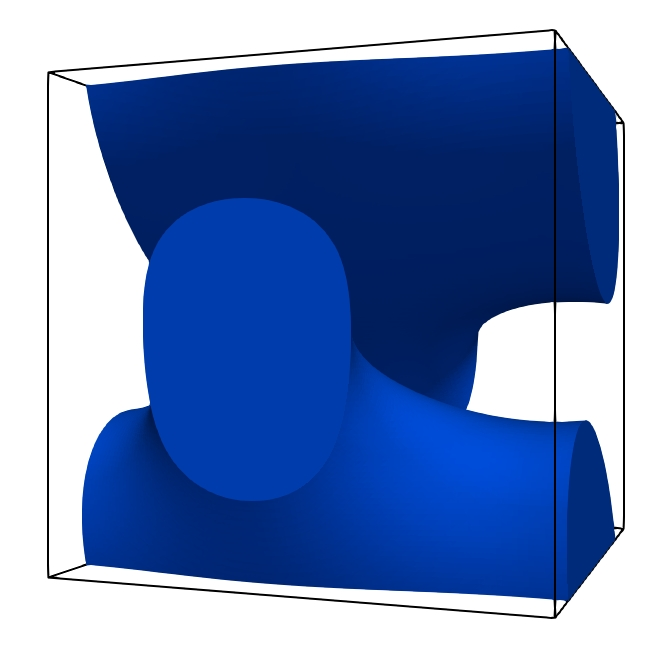
\includegraphics[width=0.95\textwidth]{Imagenes/Maxwell3D/Maxwell3D_sim/Imagenes/t_5000}
        \caption{$t = 5000$}
    \end{subfigure}
    \begin{subfigure}[t]{0.45\textwidth}
        \centering
        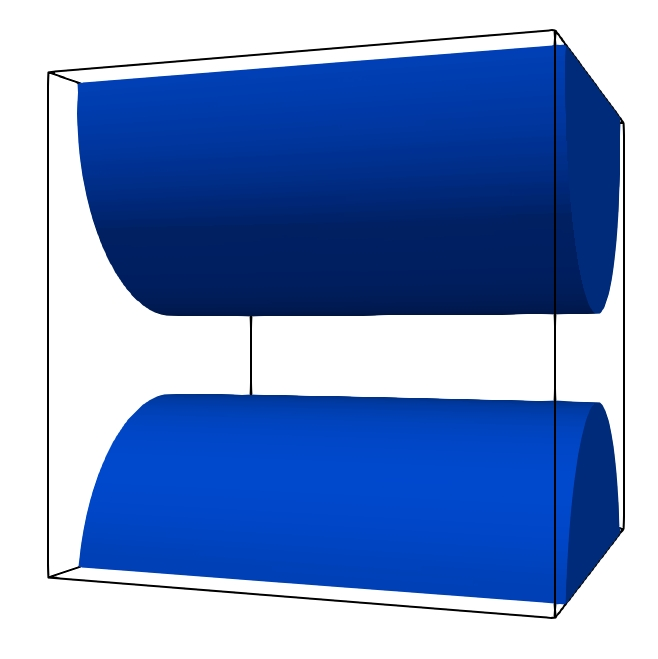
\includegraphics[width=0.95\textwidth]{Imagenes/Maxwell3D/Maxwell3D_sim/Imagenes/t_10000}
        \caption{$t = 10000$}
    \end{subfigure}        
    \caption{Evoluci\'on de una regi\'on tridimensional, peri\'odica, isot\'ermica y sin fuerzas externas, usada para verificar la regla de construcci\'on de Maxwell. La regi\'on mostrada corresponde a la fase de menor densidad.}
    \label{fig:maxwell_3d}
\end{figure}
\FloatBarrier

El modelo isot\'ermico de Xu contin\'ua con la propuesta de Li \cite{li_forcing_2012}, que consiste en modificar el t\'ermino de fuerza $\bar{\bm{S}}$ mediante la incorporaci\'on de un par\'ametro libre $\sigma$. De esta manera, $\sigma$ puede modificarse para mejorar la resoluci\'on del problema de inconsistencia termodin\'amica, lo que implica un incrmemento en la capacidad de reproducir las curvas de coexistencia asociadas a cada ecuaci\'on de estado. Este efecto puede apreciarse en la \fig{fig:vdW_coex_3D}, donde se muestran las densidades de coexistencia obtenidas empleando la ecuaci\'on de van der Waals con diferentes valores de $\sigma$ y los par\'ametros de simulaci\'on detallados en la \tb{tab:mx3D_prop}. En este caso, la elecci\'on de $\sigma=0.12$ permite reproducir con precisi\'on la curva de coexistencia de van der Waals para un amplio rango de temperaturas.

\begin{figure}[ht]
	\centering
	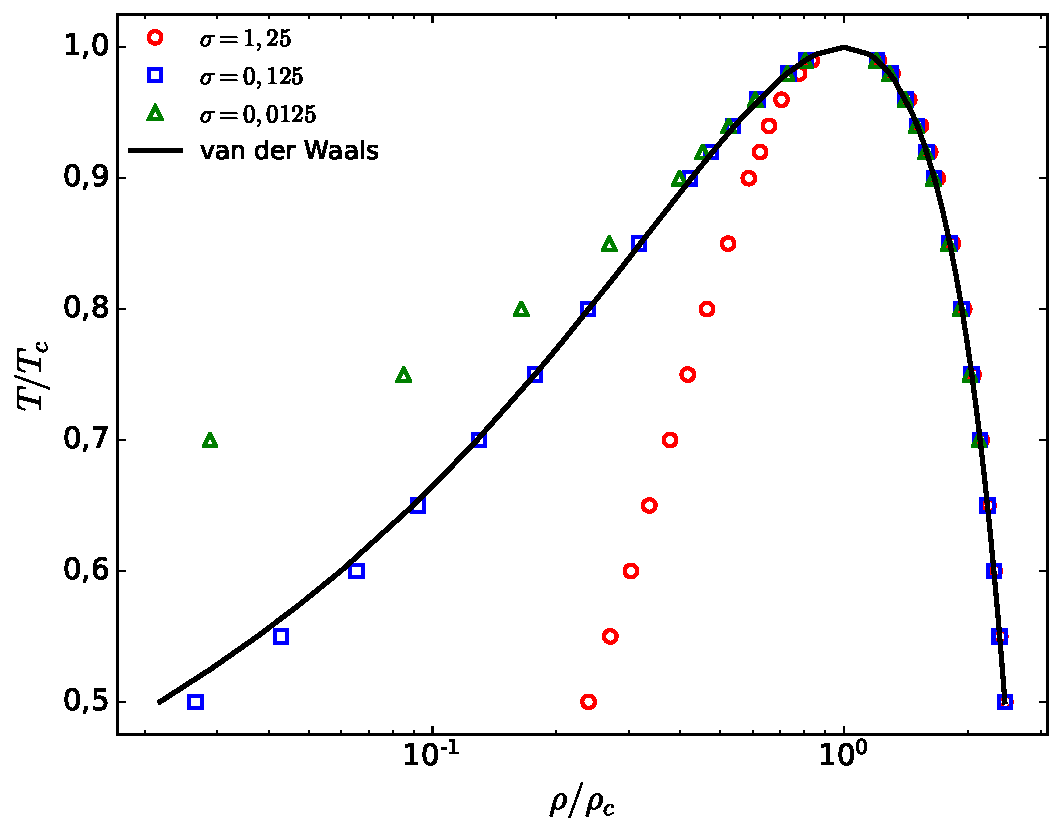
\includegraphics[width=0.75\textwidth]{Maxwell3D/Coexistencia/vdW_sigma}
	\caption{Densidades de coexistencia para la ecuaci\'on de estado de van der Waals, utilizando diferentes valores de $\sigma$. La l\'inea continua corresponde a la regla de construcci\'on de Maxwell.}
	\label{fig:vdW_coex_3D}
\end{figure}

\begin{table}[ht]
	\centering
    \begin{tabular}{c c}
	    \toprule
        \bf Propiedad & \bf Valor \\
        \midrule
        $\tau_{\rho}^{-1}$, $\tau_{j}^{-1}$ & 1.0\\
        $\tau_{e}^{-1}$, $\tau_{\zeta}^{-1}$, $\tau_{q}^{-1}$ & 1.1 \\
        $\tau_{xyz}^{-1}$ & 1.2 \\        
        $\tau_{\nu}^{-1}$ & 1.0 \\
		$a$ & 0.5 \\
		$b$ & 4 \\        
        $\kappa$ & 0 \\
        \bottomrule
	\end{tabular}
	\caption{Constantes de simulaci\'on para el problema de construcci\'on de Maxwell}
	\label{tab:mx3D_prop}
\end{table}  




\subsection{Estratificaci\'on de un fluido van der Waals}

En la \se{sec:vdWColumnHT} se utilizaron las \eqs{eq:vdw_column_red}{eq:markus_1d} para describir la distribuci\'on de densidad y temperatura en una columna de fluido van der Waals unidimensional, con temperaturas reducidas por debajo de la cr\'itica y bajo la acci\'on de una fuerza gravitacional externa. Como ya se discuti\'o extensamente en los cap\'itulos previos, la resoluci\'on de este problema constituye un excelente caso de prueba para los modelos multif\'asicos \pp{} porque permite evaluar, a partir de una \'unica soluci\'on unidimensional, la capacidad del modelo de reproducir perfiles de densidad en el seno de cada fase, la posici\'on final de la interfase o la resoluci\'on espacial de la misma.

\red{Falta decir que se usa la aproximaci\'on de $\nabla T$.}

Para llevar a cabo esta etapa de validaci\'on se realizaron simulaciones sobre una cavidad tridimensional con $H=300$ u.g. en la direcci\'on $z$ y $L=3$ u.g. en las direcciones $x$ e $y$. En este caso se consideraron las condiciones de no deslizamiento descriptas en la \se{sec:nebb_d3q15} y de temperatura fija en las caras con normal sobre $z$, junto con condiciones de periodicidad en las restantes. Los factores de relajaci\'on y dem\'as constantes de la simulaci\'on se encuentran detallados en la \tb{tab:vdwColumn3D_prop}.

\begin{table}[ht]
	\centering
    \begin{tabular}{c c}
	    \toprule
        \bf Propiedad & \bf Valor \\
        \midrule
        $\tau_{\rho}^{-1}$, $\tau_{j}^{-1}$ & $1.0$ \\
        $\tau_{e}^{-1}$, $\tau_{\zeta}^{-1}$, $\tau_{q}^{-1}$ & $1.1$ \\
        $\tau_{xyz}^{-1}$ & $1.2$ \\
        $\tau_{\nu}^{-1}$ & $1.1$ \\
		$a$ & $0.5$ \\
		$b$ & $4$ \\
		$\kappa$   & 0 \\
		$E_r (H)$  & $0.001$ \\
		$q_{0-2}$, $q_4$, $q_{6}$, $q_{8-14}$ & $1.0$ \\
		$q_{\chi}$ & $1.0$ \\
		$\alpha_1$ & $-1$ \\
		$\alpha_2$ & $1$ \\
		$c_v$      & $4$ \\
        \bottomrule
	\end{tabular}
	\caption{Constantes de simulaci\'on para el problema estratificaci\'on de un fluido van der Waals.}
	\label{tab:vdwColumn3D_prop}
\end{table}  

En una primera prueba num\'erica se fij\'o el valor de temperatura de la cara superior en $T_t = 0.99 T_c$, y se realizaron simulaciones para diferentes valores de temperatura en la cara inferior ($T_b$). Las \figs{fig:vdWColumnHT_rhor_3D}{fig:vdWColumnHT_Tr_3D} muestran las distribuciones de densidad y temperatura obtenidas para diferentes valores de $T_b$, donde se observa que la soluci\'n de lattice Boltzmann reproduce campos macrosc\'opicos con similares caracter\'isticas a los del modelo D2Q9, es decir, perfiles de densidad y temperatura similares a la soluci\'on anal\'itica en el seno del fluido, y con una interfase cuyo espesor disminuye con la temperatura. En este caso, la \lbe{} propuesta para un conjunto de velocidades D3Q15 produce una distribuci\'on de temperatura continua a lo largo de la cavidad, mientras que el espesor no nulo de la interfase no afecta significativamente a la distribuci\'on de $T$ en la zona de la separaci\'on.

\begin{figure}[ht]
	\centering
	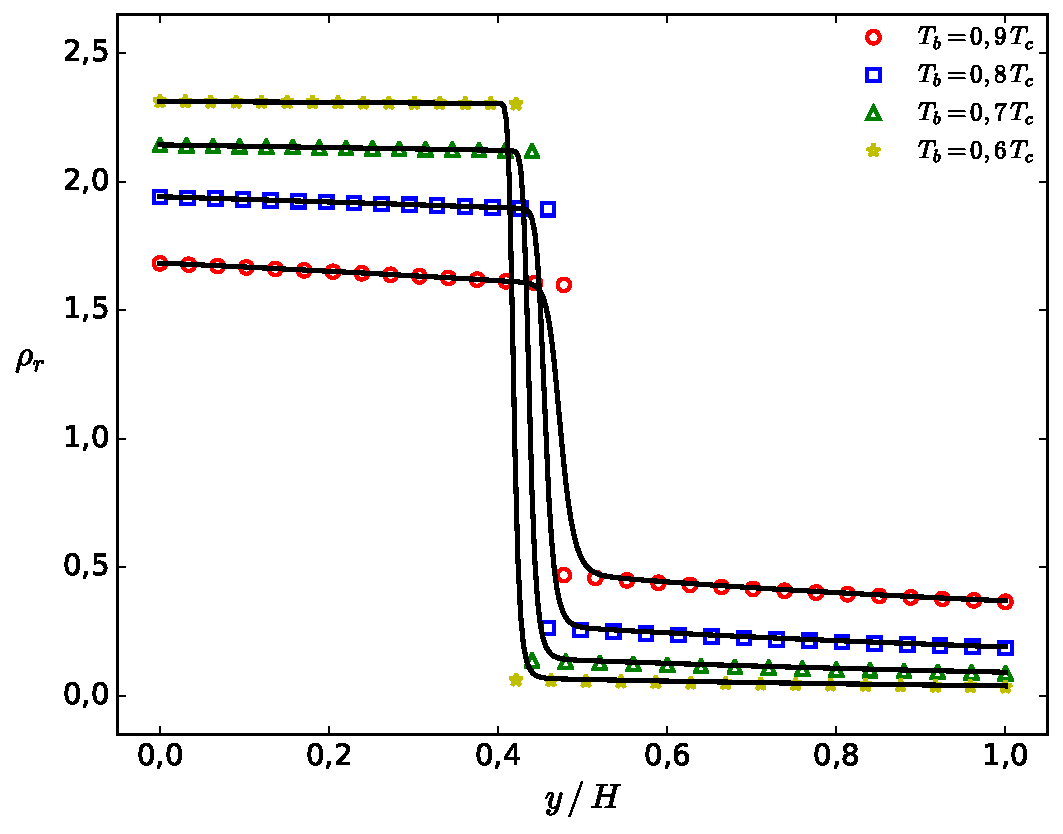
\includegraphics[width=0.75\textwidth]{vdWColumnHT_2D/CasoA/rhor_vdWcolumnHT}
	\caption{Distribuci\'on espacial de densidad en una cavidad con diferentes temperaturas en la cara inferior. Las l\'ineas continuas corresponden a simulaciones de lattice Boltzmann.}
	\label{fig:vdWColumnHT_rhor_3D}
\end{figure}

\begin{figure}[ht]
	\centering
	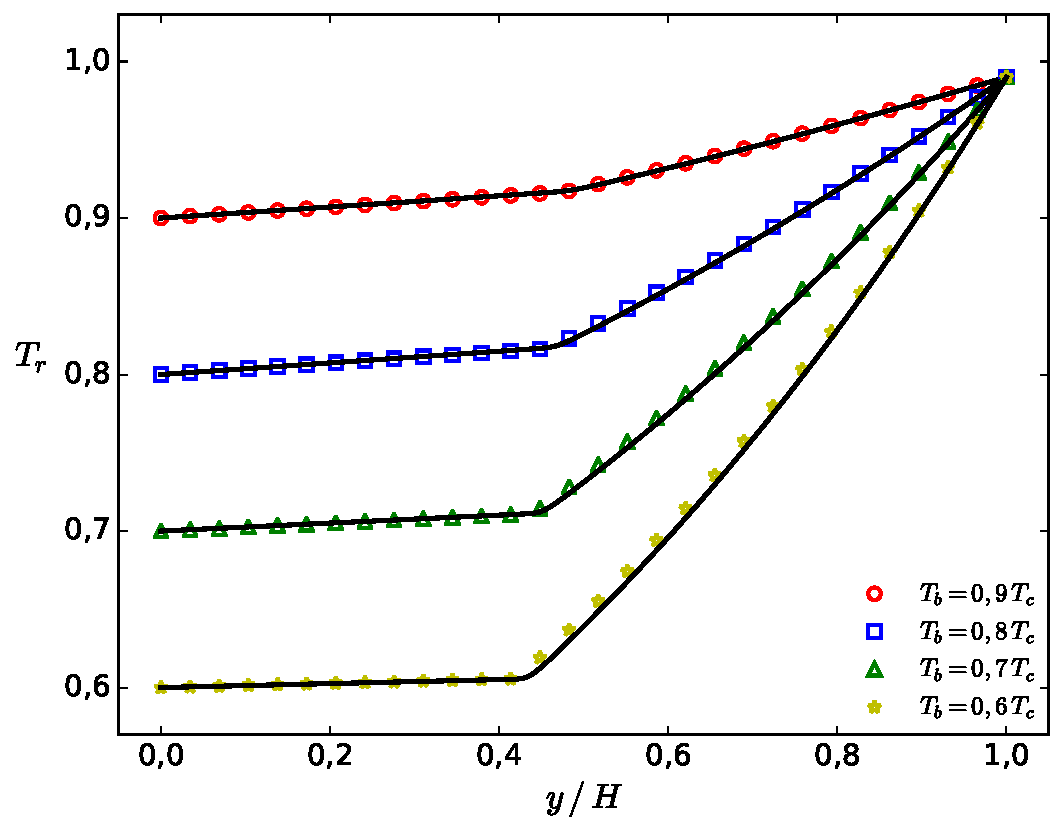
\includegraphics[width=0.75\textwidth]{vdWColumnHT_2D/CasoA/Tr_vdWcolumnHT}
	\caption{Distribuci\'on espacial de temperatura en una cavidad con diferentes temperaturas en la cara inferior. Las l\'ineas continuas corresponden a simulaciones de lattice Boltzmann.}
	\label{fig:vdWColumnHT_Tr_3D}
\end{figure}

La representaci\'on de la soluci\'on num\'erica mediante variables reducidas conduce, al igual que en el modelo D2Q9, a una concordancia entre la simulaci\'on y la soluci\'on anal\'itica que mejora con el incremento de la resoluci\'on espacial. Esta consistencia se manifiesta en los perfiles de densidad mostrados en la \fig{fig:vdWColumnHT_rhor_grilla_3D}, correspondientes a simulaciones sobre cavidades con diferentes unidades de grilla en la direcci\'on $z$, usando $T_t = 0.99 \, T_c$ y $T_b = 0.8 \, T_c$.

\begin{figure}[ht]
	\centering
	\includegraphics[width=0.75\textwidth]{vdWColumnHT_2D/CasoB/rhor_vdWcolumnHT_grilla}
	\caption{Distribuci\'on espacial de densidad en una cavidad con $T_b = 0.8 \, T_c$, $E_r(H)=10^{-3}$ y diferentes $H$. Las l\'ineas continuas corresponden a simulaciones de lattice Boltzmann.}
	\label{fig:vdWColumnHT_rhor_grilla_3D}
\end{figure}


Las constantes de la ecuaci\'on de estado juegan un papel fundamental en la precisi\'on de la simulaci\'on para describir los perfiles de densidad y temperatura a trav\'es de la interfase. Las \figs{fig:vdWColumnHT_rhor_a_eos_3D}{fig:vdWColumnHT_rhor_b_eos_3D} muestran la distribuci\'on de densidad en una cavidad con $T_t = 0.99 \, T_c$ y $T_b = 0.8 \, T_c$, obtenidas con $b=4$ y variando $a$, y con $a=0.5$ pero cambiando $b$. Puede verse que en ambos casos, incrementando $a$ o reduciendo $b$, se reduce el espesor de la interfase en unidades de grilla mientras que se mantienen los perfiles de densidad reducidos en el seno de cada fase. Por otro lado, la disminuci\'on del par\'ametro $b$ aumenta la diferencia entre las densidades de l\'iquido y vapor, mientras que el incremento de $a$ y decremento de $b$ aumenta el gradiente del potencial de interacci\'on. Ambos efectos contribuyen a mejorar la capacidad del modelo \pp{} de reproducir adecuadamente la interfase,de modo que los efectos sobre la soluci\'on adimensional son similares a los observados cuando se incrementa la resoluci\'on de grilla.

\begin{figure}[ht]
	\centering
	\includegraphics[width=0.75\textwidth]{vdWColumnHT_2D/CasoC/rhor_vdWcolumnHT_a_eos}
	\caption{Distribuci\'on espacial de densidad en una cavidad con $T_t = 0.99 \, T_c$ y $T_b = 0.8 \, T_c$. Las l\'ineas continuas corresponden a simulaciones de lattice Boltzmann con $b=4$ y distintos valores de $a$.}
	\label{fig:vdWColumnHT_rhor_a_eos_3D}
\end{figure}

\begin{figure}[ht]
	\centering
	\includegraphics[width=0.75\textwidth]{vdWColumnHT_2D/CasoD/rhor_vdWcolumnHT_b_eos}
	\caption{Distribuci\'on espacial de densidad en una cavidad con $T_t = 0.99 \, T_c$ y $T_b = 0.8 \, T_c$. Las l\'ineas continuas corresponden a simulaciones de lattice Boltzmann con $a=0.5$ y distintos valores de $b$.}
	\label{fig:vdWColumnHT_rhor_b_eos_3D}
\end{figure}




\subsection{Frente de evaporaci\'on}

La simulaci\'on del avance de un frente de evaporaci\'on, tambi\'en conocido como problema de Stefan unidimensional, puede emplearse para evaluar aquellos aspectos no cubiertos por la soluci\'on de un fluido van der Waals estratificado. En particular, la din\'amica del problema implica que la \lbe{} asociada a la ecuaci\'on de energ\'ia debe ser capaz de cuantificar adecuadamente la transferencia de masa a trav\'es de la interfase, lo que se asocia directamente con la reproducci\'on adecuada del t\'ermino dependiente de $\nabla \cdot \bm{u}$ en la ecuaci\'on de M\'arkus y H\'azi \cite{safari_consistent_2014}.

Tomando como base la soluci\'on anal\'itica descripta en la \se{sec:stefan_d2q9}, se realizaron simulaciones sobre un dominio de $L=600$ u.g. en la direcci\'on $x$ y s\'olo $H=3$ en las direcciones peri\'odicas $z$ e $y$. n todos los casos se impusieron condiciones de temperatura fija en los extremos del dominio con $T(L) = 0.8 \, T_c$, de no deslizamiento en $x=0$, y de flujo saliente (\emph{outflow}) para densidad y velocidad en $x=L$ \cite{lou_evaluation_2013}. Las constantes de simulaci\'on empleadas en las \lbe{} hidrodin\'amica y de energ\'ia se encuentran en la \tb{tab:stefan3D_prop}. 

\begin{table}[ht]
	\centering
    \begin{tabular}{c c}
	    \toprule
        \bf Propiedad & \bf Valor \\
        \midrule
        $\tau_{\rho}^{-1}$, $\tau_{j}^{-1}$ & $1.0$ \\
        $\tau_{e}^{-1}$, $\tau_{\zeta}^{-1}$, $\tau_{q}^{-1}$ & $1.1$ \\
        $\tau_{xyz}^{-1}$ & $1.2$ \\
        $\tau_{\nu}^{-1}$ & $1.1$ \\
		$a$ & $0.5$ \\
		$b$ & $4$ \\
		$\kappa$   & 0 \\
		$E_r (H)$  & $0.001$ \\
		$q_{0-2}$, $q_4$, $q_{6}$, $q_{8-14}$ & $1.0$ \\
		$q_{\chi}$ & $1.0$ \\
		$\alpha_1$ & $-1$ \\
		$\alpha_2$ & $1$ \\
		$c_v$      & $4$ \\
        \bottomrule
	\end{tabular}
	\caption{Constantes para la simulaci\'on el problema del frente de evaporaci\'on usando el modelo D3Q15.}
	\label{tab:stefan3D_prop}
\end{table} 

\red{Poner los valores correctos en la tabla}

Inicialmente, el dominio se encuentra a temperatura uniforme $T_r = 0.8$, y la distribuci\'on de densidad es uniforme e igual a la de coexistencia de la fase l\'iquida a $T_r = 0.8$. Si se deja evolucionar un sistema con esta configuraci\'on, inicialmente se produce una zona de vapor en $x=0$ sin necesidad de incluir un disparador adicional, como puede ser una peque\~na regi\'on de vapor, y la posici\'on de la interfase de desplaza hasta alcanzar $x=L$. La \fig{fig:Stefan_m1_1_3D} muestra la posici\'on de la interfase calculada usando diferentes valores de $T_w$, lo cual se refleja en distintos n\'umeros de Stefan. La evoluci\'on de la interfase mostrada en la \fig{fig:Stefan_m1_1_3D} indica que el modelo propuesto puede reproducir satisfactoriamente la estimaci\'on dada por las \eqs{eq:stefan_int}{eq:stefan_beta}, lo que implica que la transferencia de masa a trav\'es de las interfase puede ser recuperada correctamente cuando el cambio de fase est\'a governado por una ecuaci\'on de estado, sin necesidad de reconstruir la interfase o de efectuar aproximaciones adicionales.

\begin{figure}[ht]
	\centering
	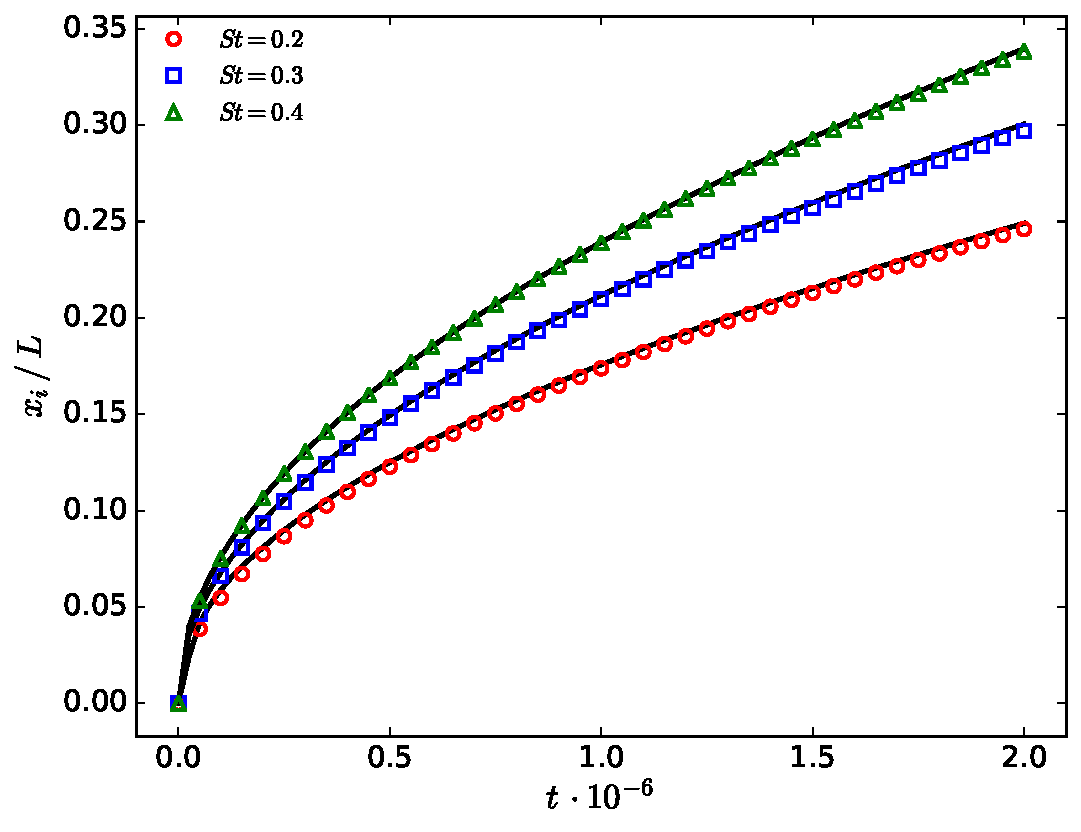
\includegraphics[width=0.75\textwidth]{Stefan/2D/CasoA/Stefan_m1_1}
	\caption{Posici\'on del frente de evaporaci\'on para diferentes n\'umeros de Stefan, con $\alpha_1 = -1$, $\alpha_2=1$ y $q_{\chi} = 1.8$. Las l\'ineas s\'olidas corresponden a las simulaciones con lattice Boltzmann}
	\label{fig:Stefan_m1_1_3D}
\end{figure}

El desarrollo de la \lbe{} para un conjunto de velocidades D3Q15 muestra que, de manera similar a lo que ocurre con el modelo para D2Q9, en este caso la conductividad t\'ermica puede modificarse alternativamente usando los par\'ametros $\alpha_1$ y $\alpha_2$ de la distribuci\'on de equilibrio $\feq{n}$, flexibilizando el uso del factor de relajaci\'on $q_{\chi}$. Para ilustrar esta caracter\'istica, se realizaron simulaciones del frente de evaporaci\'on usando $\alpha_1=-2$, $\alpha_2=2$ y $q_{\chi}=1.7143$, lo que formalmente reproduce la misma difusividad t\'ermica que $\alpha_1=-1$, $\alpha_2=1$ y $q_{\chi}=1.8$, y por lo tanto, el mismo resultado f\'isico. Como se aprecia en la \fig{fig:Stefan_m2_2_3D}, la evoluci\'on del frente de evaporaci\'on no se distingue de aquella obtenida mediante otro conjunto de par\'ametros (\fig{fig:Stefan_m1_1_3D}), lo que indica que la difusividad t\'ermica recuperada es la misma en ambos casos. Esta capacidad de usar diferentes factores de relajaci\'on para lograr un mismo valor de $\chi$ puede ser utilizada para compensar simulaciones num\'ericamente inestables.

\begin{figure}[ht]
	\centering
	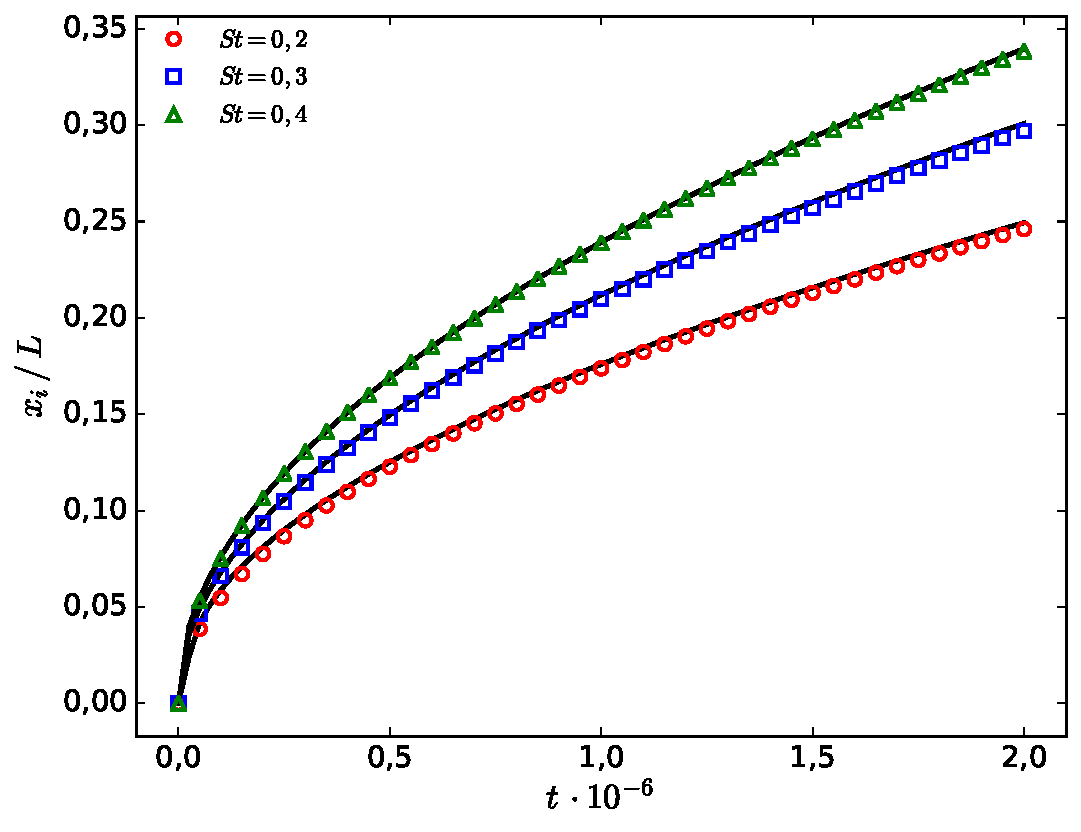
\includegraphics[width=0.75\textwidth]{Stefan/2D/CasoB/Stefan_m2_2}
	\caption{Posici\'on del frente de evaporaci\'on para diferentes n\'umeros de Stefan, con $\alpha_1 = -2$, $\alpha_2=2$ y $q_{\chi} = 1.7143$. Las l\'ineas s\'olidas corresponden a las simulaciones con lattice Boltzmann}
	\label{fig:Stefan_m2_2_3D}
\end{figure}
